\documentclass{slide}

\usepackage{changepage}
\usepackage{tabto}
% \usepackage{pgfpages}
% \setbeameroption{show notes on second screen}

\title{Serverless Architecture}
\subtitle{Software Architecture}
\author{Richard Thomas}
\date{\week{12}}

\begin{document}

\maketitle

\oxymoron{Serverless}{Logic running on someone else's server.}
\note{Developers can focus on logic, not infrastructure to deliver it.}

\definition{Backend as a Service (BaaS)}{Cloud-hosted applications or services that deliver functionality used by an application front-end.}
\note[itemize]{
    \item Front-end may be a SPA or mobile app.
    \item Back-end provides sophisticated functionality (e.g. database, machine learning, location services, authentication, \dots).
    \item Front-end ties back-end services together to deliver the application's functionality.
}

\begin{frame}{BaaS Example}
    \begin{adjustwidth}{-12mm}{-12mm}
        \centering
        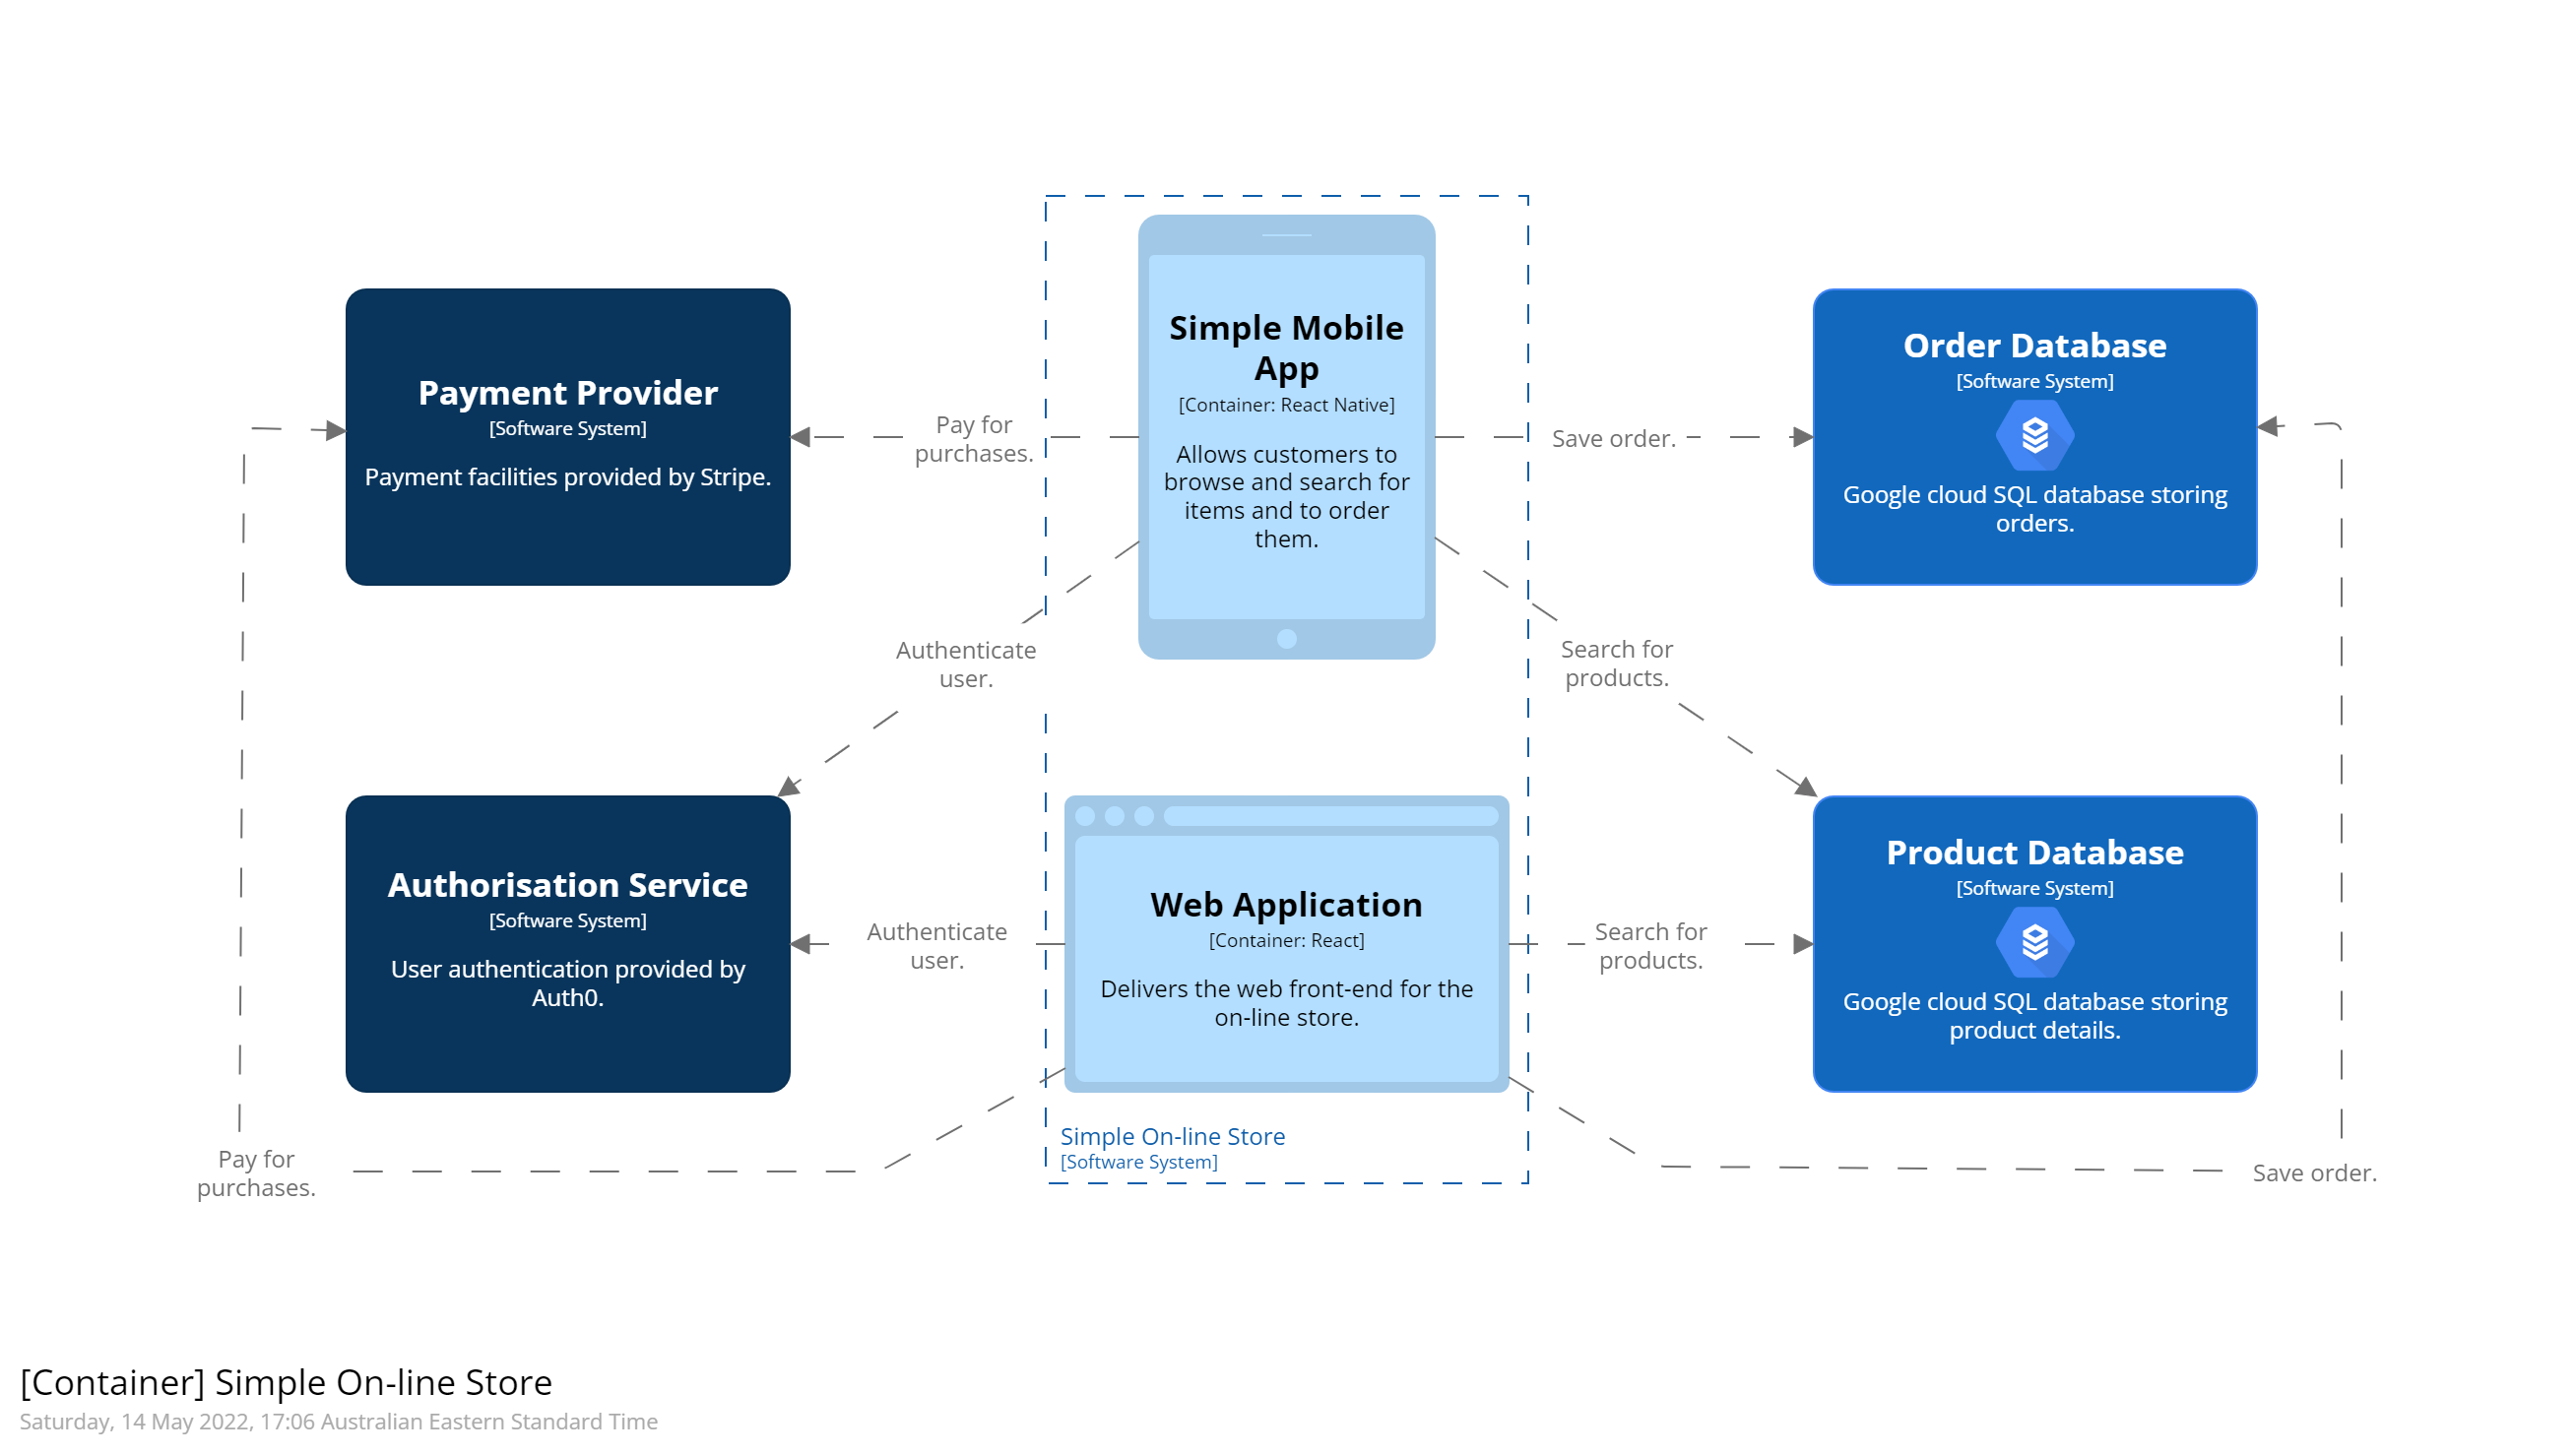
\includegraphics[trim=195 195 195 195,clip,width=0.98\paperwidth]{diagrams/baas-example.png}
    \end{adjustwidth}
\end{frame}
\note[itemize]{
    \item Example of simple system with back-end functionality delivered entirely via BaaS.
    \item Feature-rich front-ends coordinate behaviour delivered by BaaS.
    \item Consequence: Front-ends are tightly coupled to BaaS.
    \item Consequence: Front-ends are have both UI and functional behaviour logic.
    \item Front-end could have a layered design, though many SPAs don't.
}

\definition{Functions as a Service (FaaS)}{Application logic that is triggered by an event and runs in a transient, stateless compute node.}
\note[itemize]{
    \item Node may only exist for duration of function call.
    \item Server infrastructure (e.g. type of node, lifespan, scaling, \dots) are managed by hosting provider.
    \item e.g. AWS Lambda, Google App Engine, Azure Automation, \dots.
}

\begin{frame}{FaaS Example}
    \begin{adjustwidth}{-12mm}{-12mm}
        \centering
        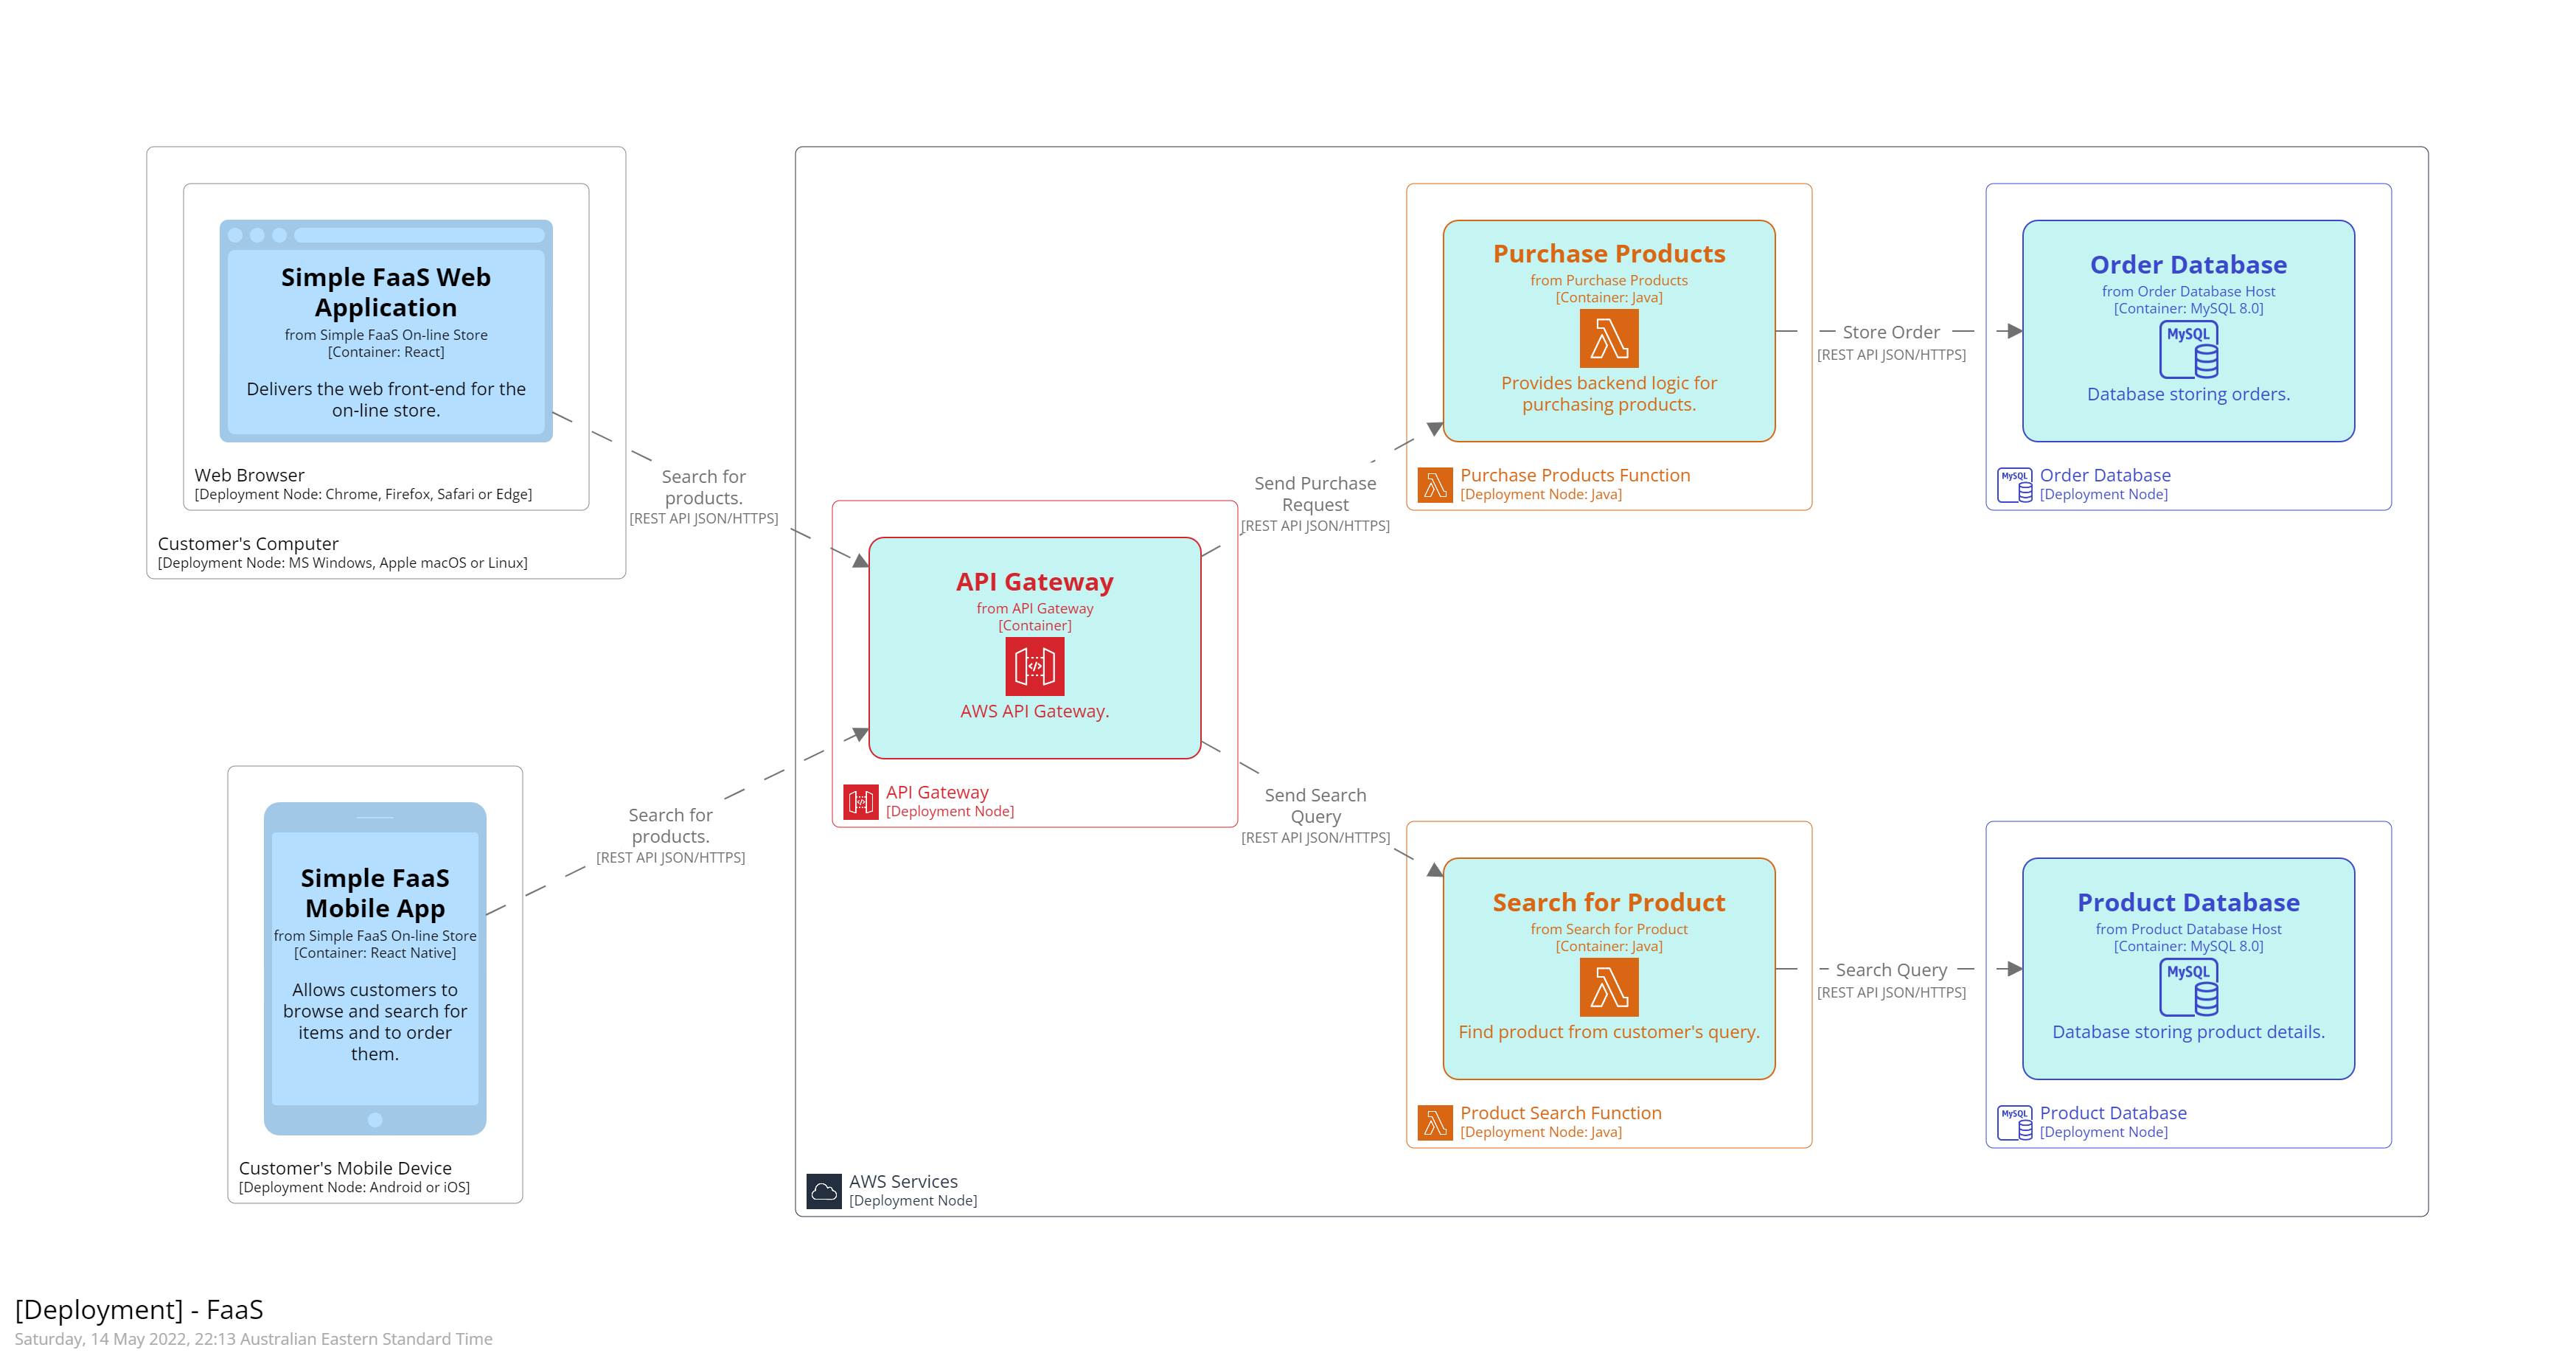
\includegraphics[trim=195 195 195 195,clip,width=0.98\paperwidth]{diagrams/faas-example.png}
    \end{adjustwidth}
\end{frame}
\note[itemize]{
    \item Example of simple system with back-end functionality delivered entirely by FaaS.
    \item Feature-rich front-ends coordinate behaviour delivered by FaaS.
    \item Front-ends invoke functions via an API.
    \item API Gateway provides some separation between front-end and functions.
    \item May allow a bit more separation between UI and logic.
}

\definition{Serverless Architecture}{Software system delivering functionality through BaaS or FaaS.}
\note[itemize]{
    \item Many people focus on FaaS when considering Serverless.
    \item Some simple Single Page Web Apps (SPA) coordinate.
    \item Front-end ties back-end services together to deliver the application's functionality.
}

\begin{frame}{Serverless Sahara eCommerce}
    \begin{adjustwidth}{-12mm}{-12mm}
        \centering
        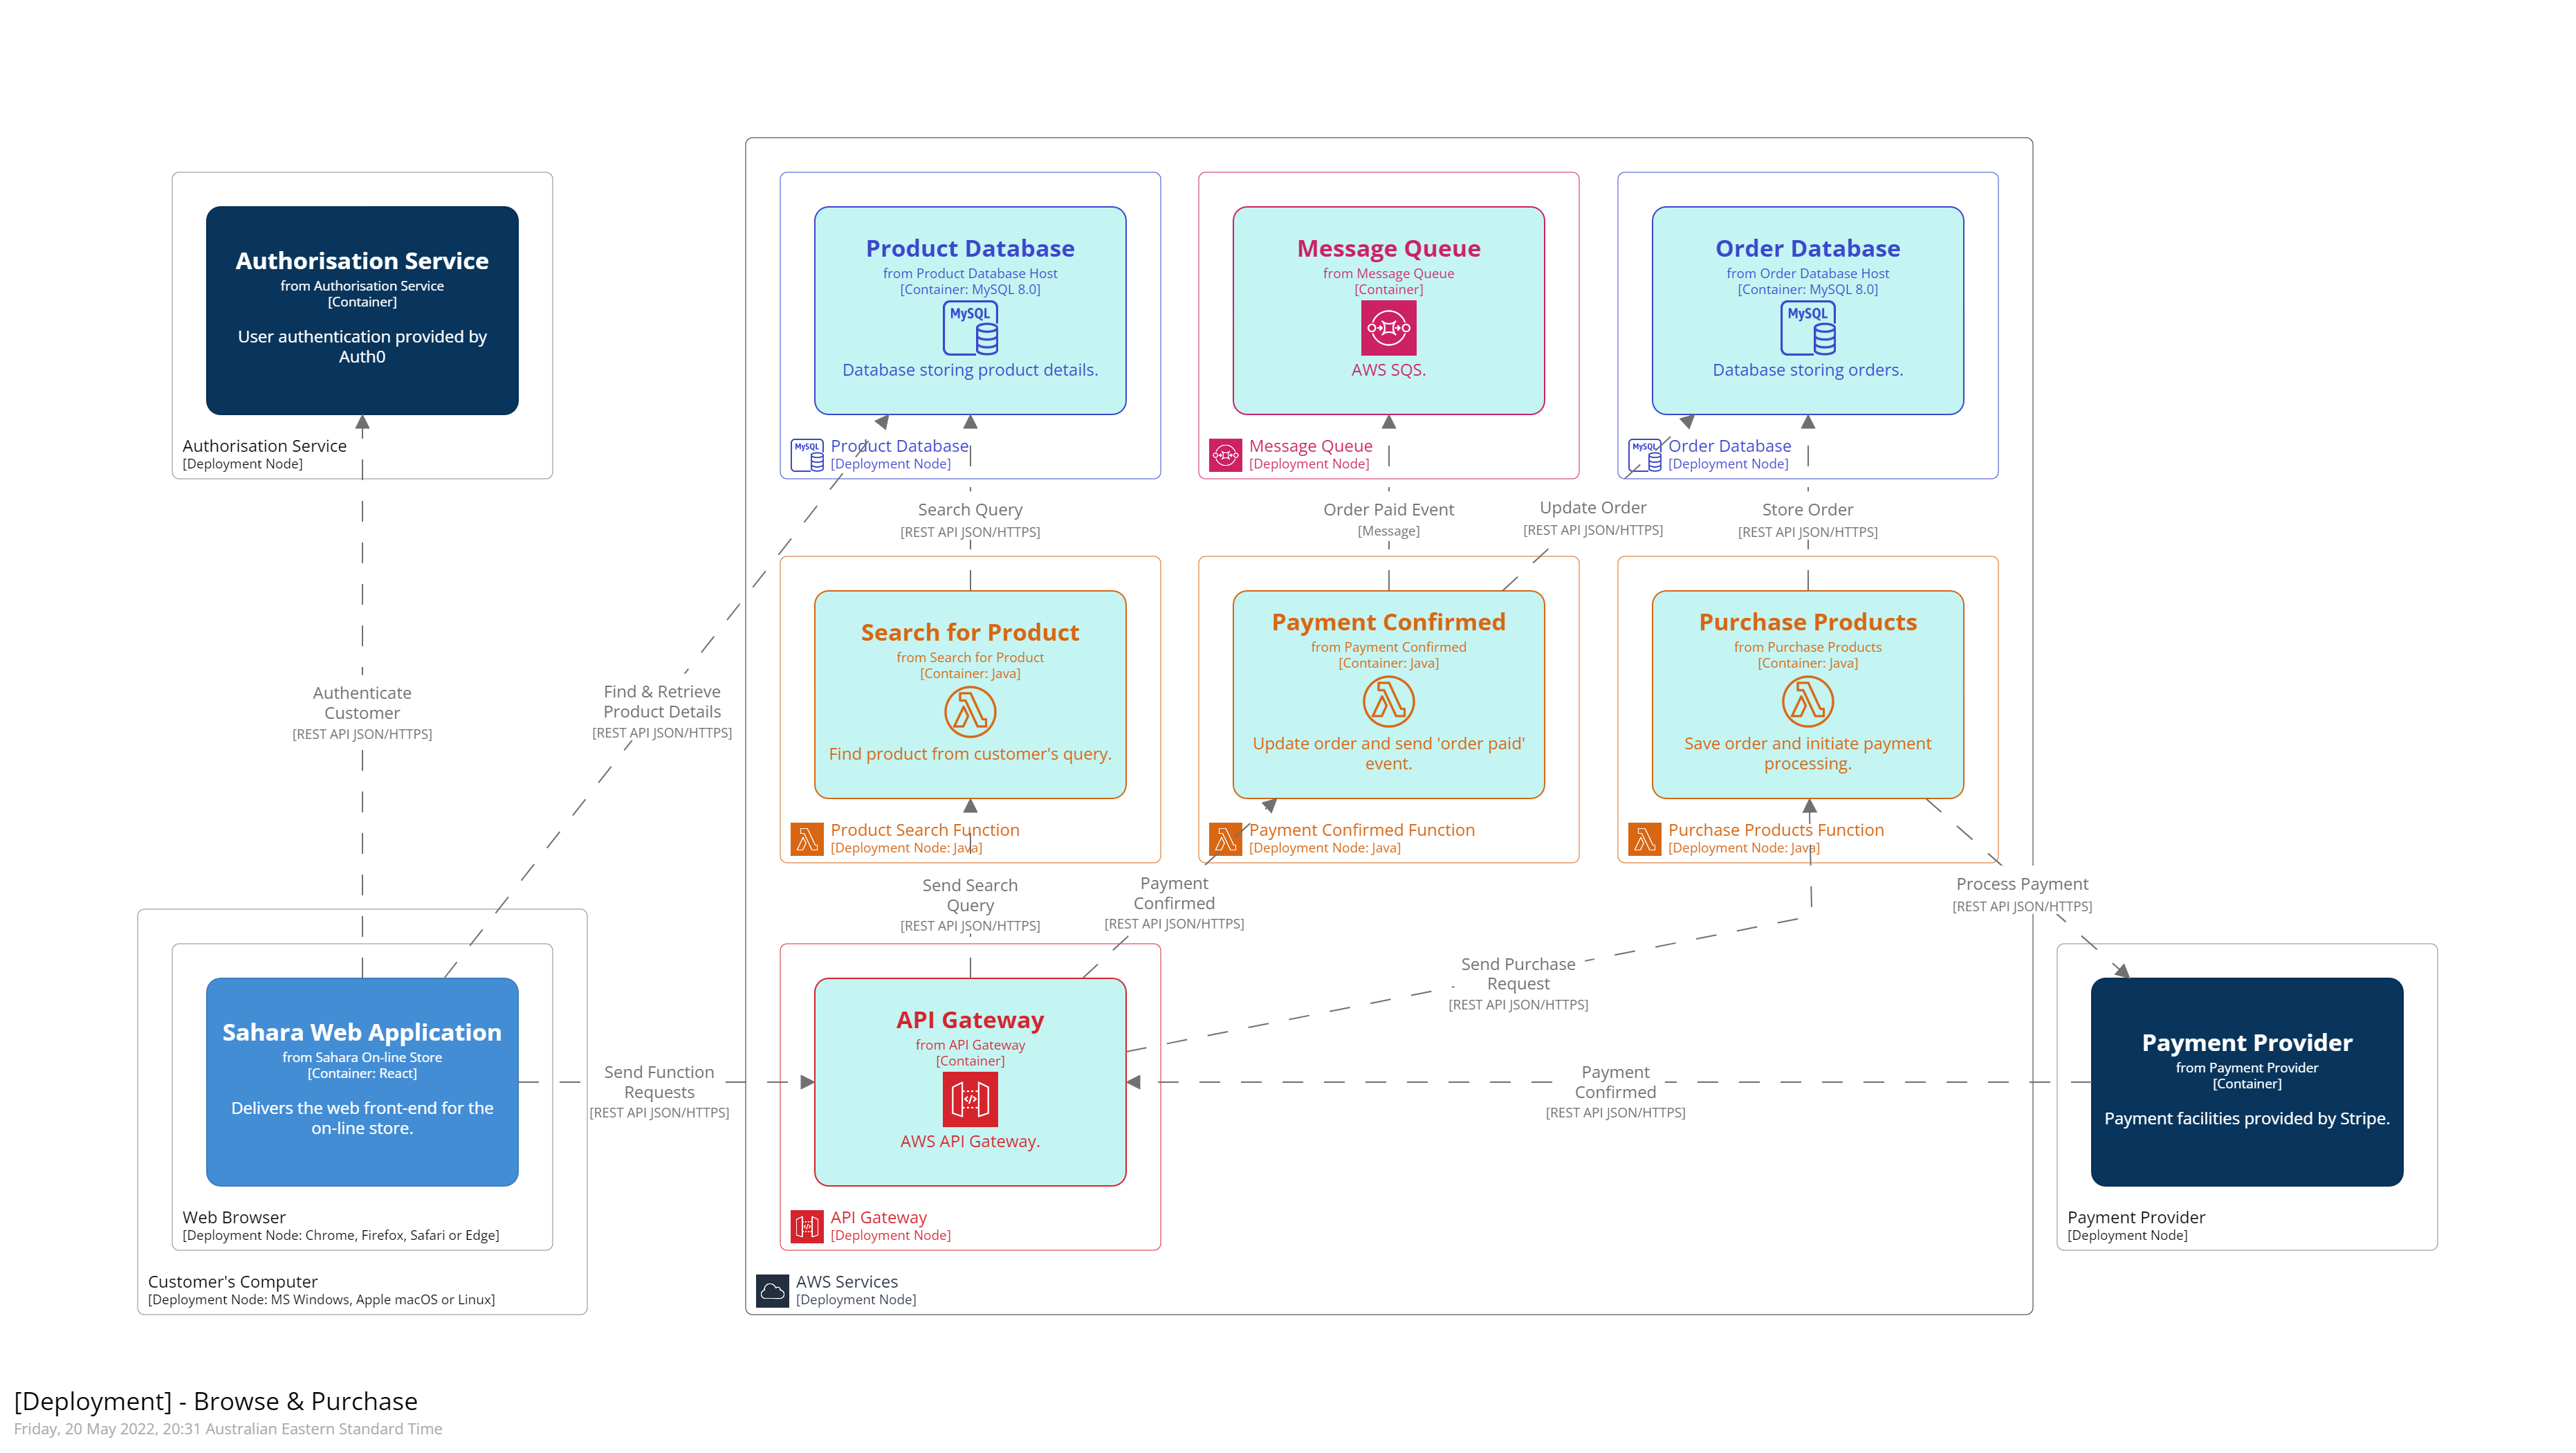
\includegraphics[trim=195 195 195 195,clip,width=\paperwidth]{diagrams/sahara-deployment-1.png}
    \end{adjustwidth}
\end{frame}
\note[itemize]{
    \item Sahara eCommerce example as a serverless app.
    \item Only browse, search and purchase are shown.
    \item Should mention that shopping cart is within the web or mobile app.
    \item Payment Confirmation event added to Queue would be picked up by a fulfillment function to pack \& send order.
    \item Once sent, another event would trigger an `order sent' function.
}

\todo{Continue Sahara Example with Steps After Diagram Above}

\begin{frame}{Pros \& Cons}
    \vspace{1mm}
    {\LARGE
    \begin{description}
        \item[Modularity] \tabto{15em}
\includegraphics[width=8mm]{../../shared/images/thumbs-up.png}
        \item[Extensibility] \tabto{15em}
\includegraphics[width=8mm]{../../shared/images/thumbs-up.png}
        \item[Reliability] \tabto{15em}
\includegraphics[width=8mm]{../../shared/images/thumbs-up.png}
        \item[Interoperability] \tabto{15em}
\includegraphics[width=8mm]{../../shared/images/thumbs-up.png}
        \item[Scalability] \tabto{15em}
\includegraphics[width=8mm]{../../shared/images/thumbs-up.png}
        \item[Security] \tabto{15em}
\includegraphics[trim=57 145 70 85,clip,width=8mm]{../../shared/images/neutral.png}
        \item[Deployability] \tabto{15em}
\includegraphics[trim=22 19 22 12,clip,width=8mm]{../../shared/images/neutral.png}
        \item[Testability] \tabto{15em}
\includegraphics[trim=22 19 22 12,clip,width=8mm]{../../shared/images/neutral.png}
        \item[Simplicity] \tabto{15em}
\includegraphics[trim=22 19 22 12,clip,width=8mm]{../../shared/images/thumbs-down.png}
    \end{description}
    }
\end{frame}

\end{document}